% ---------------------------------------------------------------------
\documentclass{article}

\usepackage{nberpreamble}
\title{\bfseries Notes on Simulating Power}
\author{\sffamily Prepared by Mauricio C\'aceres}
\date{\sffamily \today}

\usepackage{fontspec}
\fontspec{Open Sans}
\setmainfont{Open Sans Light}
% \setmathfont{Cambria Math}

\usepackage{pgfplots}  % awesome plotting
\usepackage{tikz}      % vector graphics!
\usetikzlibrary{
  arrows,
  patterns,
  positioning,
  calc,
  fit,
  intersections,
  decorations.text,
  decorations.markings,
  decorations.pathmorphing,
  shadows.blur
}

\pgfplotsset{
  compat      = newest,
  axis x line = middle,
  axis y line = center,
  tick align  = outside,
  yticklabels = {,,},
  xticklabels = {,,},
  xtick       = {0},
  ytick       = {0}
}

\renewcommand{\displayoptions}{
  % \maketitle
  % \pagenumbering{arabic}
}

% ---------------------------------------------------------------------
\begin{document}
\displayoptions

\begin{figure}[H]
  \centering
  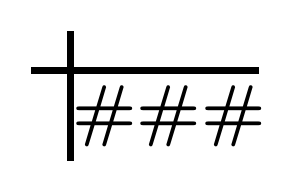
\begin{tikzpicture}[scale=1]
  \draw [line width = 2.5pt] (-0.5, 3.5) -- (-0.5, 1.85);
  \draw [line width = 2.5pt] (-1.0, 3) -- (1.90, 3);
  \node[above] at (0.75, 1.9) {\Huge\bfseries \#\#\#};
  \end{tikzpicture}
\end{figure}

%----------------------------------------------------------------------
\end{document}
